\subsubsection{Metadata}
\label{sec:model_metadata}

\paragraph{}
A data parser may, if appropriate, define experimental \texttt{outcomes} associated with the newly parsed datafile. For example an AffyBatch may contain the results of multiple arrays run under different conditions, each array is registered with the database as a different \texttt{outcome}. These outcomes may then be associated with metadata describing the levels of factors, or values of continuous variables used in their generation. All the possible outcomes are registered with the experiment and datafiles belonging to that experiment can also be annotated with all or a subset of those outcomes. 

%It should be noted that once the experiment has had outcomes defined, they cannot currently be redefined or added to by later parsing processes.

\paragraph{}
The ROME model captures only the metadata pertinent to the statistical analysis of the data, which comprises the independent variables under examination and the values of those variables used to generate each experimental outcome. Discrete variables are modelled by the \texttt{factor} and \texttt{level} tables in the database. Continuous variables are modelled by the \texttt{cont\_var} table. The structure of the metadata section of the database is outlined in figure \ref{fig:metadata_mod}. 

\begin{figure}
\centering
\caption{Metadata Model Overview}\label{fig:metadata_mod}
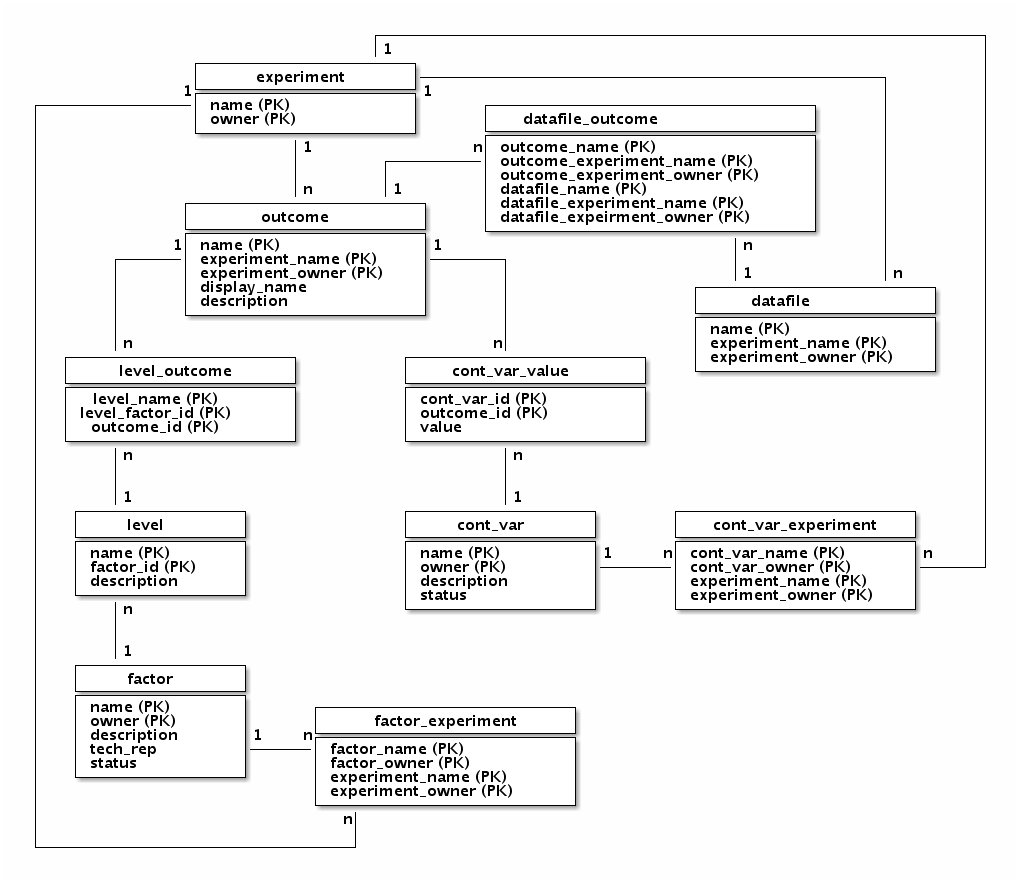
\includegraphics[scale=0.45]{images/metadata}
\end{figure}

\paragraph{}
Factors have both their name and the user who owns the factor as a primary key, which means a user can define as many factors as they like, but they must have unique names, hopefully encouraging them to reuse factors across multiple experiments which will make cross-experimental analysis easier in future. Eventually, the plan is to integrate ontologies into the metadata definitions, providing users with the option to use standardised descriptions of factors such as developmental stage, tissue type or anatomical position. Again this will enable meaningful cross-experimental analyses.
